\chapter{Implementation in das Dietrich Projekt}

In diesem Kapitel wird die Implementation ins Dietrich-Projekt genauer erläutert.

\section{Vorbereitung}

Zuerst muss der ElasticSearch Client in der Docker-Compose hinzugefügt werden. Die folgenden Vergleiche wurden in einem Docker-System gemacht mit Remote-Verbindung zur Datenbank und ElasticSearch. 

\subsection{ElasticSearch}

Zuerst soll der Lemma-Query der auch schon zum Testen in finaler Fassung in das Dietrich-Online Projekt integriert werden.

Zu Beginn muss dafür ein API-Key generiert werden, um Zugriff auf die benötigten Indices zu erhalten. Dies kann entweder über die Entwicklerkonsole oder eine Curl Abfrage geschehen \ref{lst:elaApi}. Mit diesen Key und der CA ist es nun möglich Anfragen an das ElasticSearch zu stellen.

\begin{lstlisting}[language=XML, frame=single, label={lst:elaApi}] 
    POST /_security/api_key
    {
      "name": "dietrich-webiste",
      "role_descriptors": { 
        "role-a": {
          "cluster": ["all"],
          "index": [
            {
              "names": ["dietrich_*"],
              "privileges": ["read"]
            }
          ]
        }
      }
    }
\end{lstlisting}


\subsection{Einbindung in Dietrich-Online}

Die Einbindung in das Dietrich-Online Projekt lief über KACKE

\subsubsection{Indexierung}

Da nun nicht einfach nur die Daten in das System eingepflegt werden, wurde diesmal auf die Indexierung mehr Wert gelegt. Damit Arrays ordentlich abgebildet werden, musste in der Logstash Datei Daten richtig aggregiert werden. 


//TODO RUBY


\subsection{Vergleich}

Für den Vergleich wurde zum einen 100 mal die Geschwindigkeit getestet, um die Daten in weiterverarbeitbarer Form zu bekommen.
Dafür wurden die beiden Methodenaufrufe, welche die Query generieren und ausführen, mit einem Timer umhüllt. Die erste Methode holt sich dabei alle Ids von den benötigten Lemmata und die zweite baut alle Daten zusammen, welche zur Anzeige benötigt werden. Als Framework wird für die Querys Doctrine verwendet, was sich auch um die Datenerhaltung kümmert.

\begin{lstlisting}[language=PHP, frame=single, label={lst:vglDb}] 
  ini_set('max_execution_time', 3000);

  $timeAcc = 0;
  for ($i = 0; $i < 100; $i++) {
    $time_start = microtime(true);

    $lemmas   = $this->findLemmaByCharacter($character, $filter);
    $results  = $this->findLemmaById($lemmas);

    $time_end = microtime(true);
    $time     = $time_end - $time_start;
    $timeAcc     += $time;
    echo $time.'<br/>';
  }
  
  echo 'Combined Time'.$timeAcc / 100 .'<br/>';
  die;
\end{lstlisting}

Bei ElasticSearch sieht der Query ähnlich aus. Allerdings wird hierbei ein Array generiert und es wird nur eine Abfrage gestellt. 

Bei dem Vergleich kamen die folgenden Durchschnittswerte zustande:
\begin{table} %[hbtp]
	\centering
		\begin{tabular}{l | l }
		    \textbf{System} & \textbf{Zeit} \\
        \hline
        MariaDB + Doctrine & 3.49 \\
        ElasticSearch      & 1.45  \\
		\end{tabular}
    \caption{Vergleich der Laufzeit zur Abfrage aller Daten für Buchstabe S der Lemma-Administration (15.846 Einträge)}
    \label{vlgTimeDBvsEla}
\end{table}


\begin{figure}
	\centering
	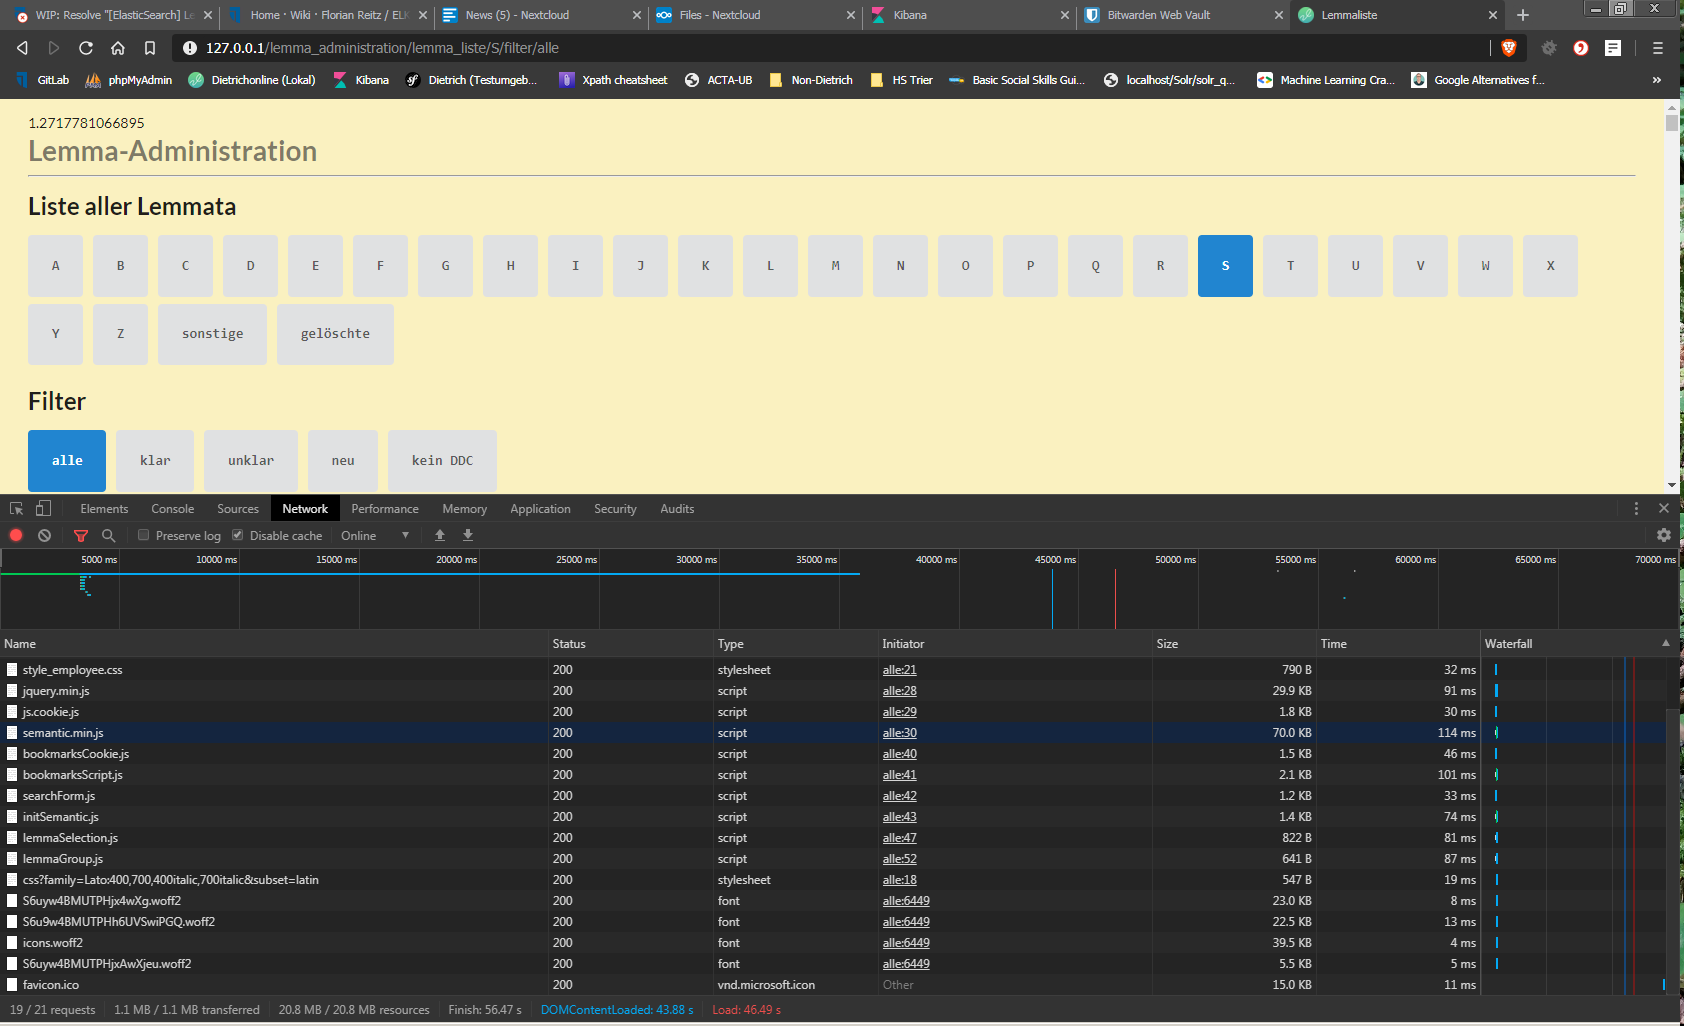
\includegraphics[width=1\linewidth]{images/setup/query/time_prod_ela.png}
	\caption{Seite zu Erstellung von Rechte-Rollen}
	\label{img:timeProdEla}
\end{figure}

\begin{figure}
	\centering
	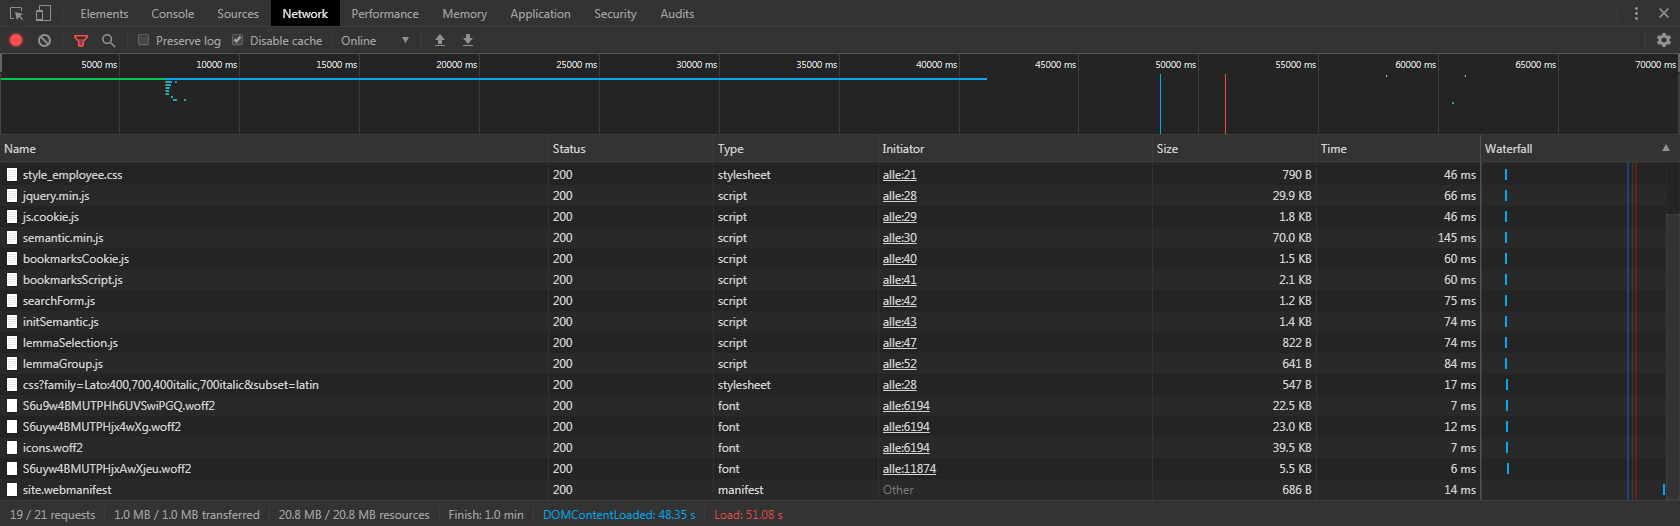
\includegraphics[width=1\linewidth]{images/setup/query/time_prod_db.png}
	\caption{Seite zu Erstellung von Rechte-Rollen}
	\label{img:timeProdDb}
\end{figure}



\begin{lstlisting}[language=PHP, frame=single, label={lst:queryEla}] 

  //Create Client with basic Params

  $mustNotQueries = [];
  $filters        = [];
  $mustQueries    = [];

  if ($character === LemmaEntity::NOT_A_TO_Z_CHARACTER) {
      $mustQueries[] = ['regexp' => ['bezeichnung.keyword' => 
        ['value' => '@&~(^[a-zA-Z].+)', 'flags' => 'ALL']]];
        
      $filters[]     = ['term' => ['ist_geloescht' => false]];
  } elseif ($character === LemmaEntity::DELETED) {
      $filters[] = ['term' => ['ist_geloescht' => true]];
  } else {
      $mustQueries = ['prefix' => ['bezeichnung.keyword' => "$character"]];
      $filters[]   = ['term' => ['ist_geloescht' => false]];
  }

  switch ($filter) {
      case self::STATUS_FILTER_KLAR:
          $filters[] = ['term' => ['bstatusbezeichnung' => 'klar']];
          break;
      //[Other Filters]
  }

  $params['body']['query']['bool']['must']     = $mustQueries;
  $params['body']['query']['bool']['must_not'] = $mustNotQueries;
  $params['body']['query']['bool']['filter']   = $filters;

  return $client->search($params)['hits']['hits'];

\end{lstlisting}

DEr query hat must, should and shouldnt

Anders als bei der Test Query \ref{lst:phpElastic} wurde bei dieser Query der Filter Prefix verwendet. Dies liegt daran, dass Praefix schneller agiert als ein Wildcard Query.